\documentclass[12pt,letterpaper]{article}

\usepackage[authoryear]{natbib}
\usepackage{times} 
\usepackage{amsmath,amsfonts}
\usepackage{graphicx}
\usepackage{setspace}
\usepackage{indentfirst}
\usepackage{url}

% revise margins
\setlength{\headheight}{0.0in}
\setlength{\headsep}{0.0in}
\setlength{\topmargin}{0.0in}
\setlength{\textheight}{8.9in}
\setlength{\footskip}{0.4in}
\setlength{\oddsidemargin}{0.0in}
\setlength{\evensidemargin}{0.0in}
\setlength{\textwidth}{6.5in}

\setlength{\rightskip}{0pt plus 1fil} % makes ragged right

%bibliography format
\usepackage[authoryear]{natbib}
\bibpunct{(}{)}{;}{a}{}{,}

\newcommand{\LOD}{\text{LOD}}
 
% hanging environment for Figure legends
\newenvironment{hanging}
{\begin{list}{}
        {\setlength{\labelwidth}{0in}
         \setlength{\leftmargin}{1em}
         \setlength{\itemindent}{-1em}
        }
}
{\end{list}}

\begin{document}
\setstretch{2.0}

\vspace*{8mm}
\begin{center}

\textbf{\Large Mapping quantitative trait loci %\\[18pt] 
onto a phylogenetic tree}
 
 
\bigskip \bigskip \bigskip \bigskip 
 
{\large Karl W. Broman$^{*,1}$, Sungjin Kim$^{\dagger,2}$, \'Saunak
  Sen$^\ddagger$,\\ 
C\'ecile An\'e$^{\dagger,\S}$, Bret A. Payseur$^{**}$}

\bigskip \bigskip

$^*$Department of Biostatistics and Medical Informatics,
$^\dagger$Department of Statistics, $^{\S}$Department of Botany, and $^{**}$Laboratory of
Genetics, University of Wisconsin--Madison, Madison, Wisconsin
53706; $^\ddagger$Department of Epidemiology and Biostatistics, University
of California, San Francisco, San Francisco, California 94107
\end{center}


\vfill

\hfill 
{\footnotesize 28 Jun 2012}

\newpage

\noindent \textbf{Running head:} Mapping QTL onto a tree


\bigskip \bigskip \bigskip

\noindent \textbf{Key words:} QTL, phylogenetic tree, evolution,
multiple crosses, combining crosses



\bigskip \bigskip \bigskip

\noindent \textbf{$^1$Corresponding author:}

\begin{tabular}{lll}
 \\
 \hspace{1cm} & \multicolumn{2}{l}{Karl W Broman} \\
 & \multicolumn{2}{l}{Department of Biostatistics and Medical Informatics} \\
 & \multicolumn{2}{l}{University of Wisconsin--Madison} \\
 & \multicolumn{2}{l}{1300 University Ave, Rm 4710 MSC} \\
 & \multicolumn{2}{l}{Madison, WI 53706} \\
 \\
 & Phone: & 608--262--4633 \\
 & Fax: & 608--265--7916 \\
 & Email: & \verb|kbroman@biostat.wisc.edu|
\end{tabular}


\bigskip \bigskip \bigskip

\noindent \textbf{$^2$Current address:} Biostatistics and
Bioinformatics Shared Resource, Winship Cancer Institute, Emory
University, Atlanta, Georgia 30322


\newpage



\centerline{ABSTRACT} 
  
Despite advances in genetic mapping of quantitative traits and in
phylogenetic comparative approaches, these two perspectives are rarely
combined.
The joint consideration of multiple crosses among related taxa
(whether species or strains) not only allows more precise mapping of
the genetic loci (called quantitative trait loci, QTL) that contribute
to important quantitative traits, but also offers the opportunity to
identify the origin of a QTL allele on the phylogenetic tree that
relates the taxa.  We describe a formal method for combining
multiple crosses to infer the location of a QTL on a tree.  We further
discuss experimental design issues for such endeavors,
such as how many crosses are required and which sets of crosses are
best. Finally, we explore the method's performance in computer
simulations, and we
illustrate its use through application to a set of four mouse
intercrosses among five inbred strains, with data on HDL cholesterol.


\newpage
\centerline{INTRODUCTION}

The analysis of experimental crosses to identify the genetic loci
(called quantitative trait loci, QTL) that contribute to variation in
quantitative traits has become a standard approach in evolutionary
biology. The properties of the QTL responsible for phenotypic
differences between populations or species---including the number of
QTL, their effect sizes, and their modes of action---provide insights
into the mechanisms of evolution. QTL data have been brought to bear
on a wide range of evolutionary processes, including adaptation
\citep{Doebley1991, Bradshaw1998, Orr1998, Mauricio2001, Peichel2001,
  Rieseberg2002, MitchellOlds2007, Steiner2007, Hall2010} and
speciation \citep{Bradshaw1995, Moehring2006, Oka2007, Shaw2007,
  Moyle2008, McDermott2011, White2011}.

By modeling the distribution of trait values across a tree,
phylogenetic comparative methods also help to reconstruct the dynamics
of phenotypic evolution. These approaches address several key issues,
including the values of traits in ancestors \citep{Schluter1997,
Pagel1999, Garland2000, Pagel2004}, rates of
phenotypic evolution \citep{Garland1992, Venditti2011}, the
connection between trait evolution and speciation/extinction
\citep{Maddison2007, Fitzjohn2009}, and the role of natural selection
vs. genetic drift \citep{Hansen1997, Freckleton2006}.

Despite the successful application of QTL mapping and phylogenetic
comparative methods to fundamental questions in evolutionary biology,
the two frameworks are rarely integrated. Methods that combine the
portraits of genetic architecture obtained from QTL mapping with the
logic of phylogenetic comparisons would offer several benefits. First,
QTL data would provide a mechanistic basis for the dynamics of
phenotypic evolution uncovered by phylogenetic comparative
approaches. Although trait shifts along trees are caused by mutations,
the methods for reconstructing these shifts do not currently
incorporate genetic information.

Second, situating QTL data within a phylogenetic framework would
directly account for the statistical dependencies that accompany any
mapping comparison among three or more taxa. The tree connecting the
species used in genetic mapping constrains the configurations of
shared and divergent QTL that are possible, but this information is
currently ignored by most QTL mapping methods.

Most importantly, a combined method could reveal the history of
genetic differences between species. The mutations that underlie QTL
occur along a phylogeny. Assigning these mutations to branches of the
tree would pinpoint their evolutionary origins and allow testable predictions
regarding the temporal accumulation of mutations 
\citep{Moyle2009}.

The ability to assign QTL to branches of phylogenetic trees would
benefit genetic research beyond evolutionary biology. Collectively or
individually, researchers often map QTL for the same phenotype in
multiple sets of strains, especially in agricultural and biomedical
model organisms. In addition to refining QTL position \citep{Li2005},
joint analysis of these crosses can pinpoint the genetic backgrounds
(strains) on which QTL arose, providing further insights into the
genetic architecture of traits involved in food quality or disease.

To envision the problem, consider the tree in
Figure~\ref{fig:tree}, and imagine the presence of a single diallelic
QTL.  The mutant allele at the QTL could have arisen in one of five
possible locations on the tree, and each location is associated with a
particular partition of the four taxa into two groups (those with the
``high'' allele, and those with the ``low'' allele).  For each such
partition, the QTL will segregate in a different subset of the
possible crosses between pairs of taxa.  Throughout, 
we focus solely on unrooted trees.  The two edges on either side of
the root in Figure~\ref{fig:tree}, labeled 5, cannot be
distinguished.  Also, a mutation arising above the root cannot be
distinguished from the null model of no QTL.

With data on multiple crosses, the simplest approach to identify the
location on the tree at which a QTL arose is to compare the pattern of
presence and absence of the QTL in the individual crosses and match
that to the ideal (see the table in Figure~\ref{fig:tree}).  We describe
a more formal approach, combining ideas from 
\citet{Li2005}, regarding the joint analysis of multiple crosses, with
ideas from \citet{MacdonaldLong2007}, regarding partitioning
multiple QTL alleles into two groups.

We discuss experimental design issues for such endeavors,
such as how many crosses are required and which sets of crosses are
best; explore the method's performance in computer simulations; and
illustrate its use through application to a set of four mouse
intercrosses among five inbred strains, with data on HDL cholesterol.



\clearpage

\centerline{METHODS}

To develop methods for mapping a QTL to a phylogenetic
tree, we begin with several simplifying assumptions: The taxa are
represented by inbred lines, the tree relating the taxa is known
without error,
the quantitative trait of interest is affected by a single
diallelic QTL, and there are no background effects (i.e., 
the effect of the QTL is the same in the different crosses in which it
is segregating).  We consider the case of intercrosses among
pairs of taxa, consider only autosomal loci, and assume a common
genetic map.

The basic idea, illustrated in Figure~\ref{fig:tree}, is that each
possible location for the origin of a diallelic QTL on the tree
corresponds to a different partition of the taxa into two groups, with
the two groups corresponding to the two QTL alleles.  For different
partitions, the QTL will segregate in different sets of crosses.
In the case of very large crosses, with each having high power to
detect the QTL, if present, we could simply consider the crosses
individually and use the pattern of presence/absence of QTL to
identify the correct partition of the taxa.  Note that one does
not need data on all possible crosses.  For the case illustrated in
Figure~\ref{fig:tree}, with four taxa, it would be sufficient to
consider the crosses A $\times$ B, A $\times$ C, and B $\times$ D, as
with just these three crosses, the five possible partitions have
distinct patterns of presence/absence of the QTL.  In the following,
we focus on partitions of the taxa into two groups, in place of
locations of the QTL on the tree.

Given limited resources and crosses of limited size, there will be
incomplete power to detect the QTL in a given cross, and so the naive
approach based on the presence or absence of the QTL in the different
crosses will likely be misleading.  A more formal approach, in which
the likelihoods for the different possible partitions are evaluated
and compared, will provide a clear assessment of the evidence for the
different locations for the QTL on the tree.  

Consider a particular location in the genome as the site of a putative
QTL, and consider a particular partition of the taxa into two QTL
alleles.  We assume a linear model with normally distributed errors
$$y_{ij} = \mu_i + \alpha a_{ij} + \delta d_{ij} + \epsilon_{ij}$$ 
where $y_{ij}$ is the phenotype for individual $j$ in cross $i$,
$\mu_i$ the average phenotype in cross $i$, $\alpha$ and $\delta$ are
the additive and dominance effects of the QTL, respectively,
and the $\epsilon_{ij}$ are independent and identically distributed
normal$(0, \sigma^2)$.  The $a_{ij}$ and $d_{ij}$ denote encodings of
the QTL genotypes, with $a_{ij} = d_{ij} = 0$ if the QTL is not
segregating in cross $i$.  For convenience, we will call the two QTL
alleles defined by the partition as the high allele (H) and the low
allele (L), though we won't actually constrain the high allele to
increase the phenotype.  If the QTL is segregating in cross
$i$, then we take $a_{ij} = -1, 0, \text{ or } +1$, if individual $j$
has QTL genotype $g_{ij} =$ LL, HL or HH, respectively, and $d_{ij} = 1$ if
individual $j$ has QTL genotype HL and $d_{ij} = 0$ otherwise.

For most putative QTL locations, the QTL genotypes will not be
observed, but we may calculate (e.g., by a hidden Markov model), the
conditional probabilities of the QTL genotypes given the available
multipoint marker genotype data, 
$p_{ijk} = \Pr(g_{ij} = k | \boldsymbol{M}_{ij})$.  It is critical
that we have a common map for the set of crosses, so that a putative
QTL location is clearly defined in all crosses.  It is not necessary,
however, that the same markers be used in all crosses, or that they be
informative in all crosses.  We may then use
standard interval mapping \citep{Lander1989} or an approximation such
as Haley-Knott regression \citep{Haley1992} to fit the model, 
estimate the parameters $\mu_i$, $\alpha$, $\delta$, and $\sigma^2$,
and calculate a LOD score, $\LOD_\pi(\lambda)$, where $\pi$ denotes the
partition of the taxa and $\lambda$ denotes the
location of the putative QTL.  The LOD score is the log$_{10}$
likelihood comparing the hypothesis of a single QTL at that location
to the null hypothesis of no QTL but with the multiple crosses allowed to
have separate phenotypic means, that is $y_{ij} \sim
\text{normal}(\mu_i, \sigma^2)$.  

This analysis is just as in \citet{Li2005}, in that one recodes the
genotypes in the crosses in which the QTL is segregating, stacks them
on top of one another, as if they were a single intercross, and performs interval mapping
with cross indicators as additive covariates.  The only 
difference is that we are considering all possible partitions of the
taxa, while \citet{Li2005} assumed a particular one.  
There is one
technicality: the crosses in which the QTL does not segregate also
need to be included in the likelihood, and they contribute to the
estimate of the residual variance.  

We thus consider each possible partition, $\pi$, one at a time, and
scan the genome to obtain a set of LOD curves, $\LOD_\pi(\lambda)$.
We summarize these at the chromosome level, calculating the maximum LOD
score for partition $\pi$ on chromosome $i$, $M_{\pi i} =
\max_{\lambda \in i} \LOD_\pi(\lambda)$.  The maximum on chromosome
$i$, $\max_\pi M_{\pi i}$, indicates the evidence for a QTL on
chromosome $i$.  

To evaluate the relative support of the different partitions, we use
an approximate Bayes procedure.  Assuming the
presence of a single diallelic QTL on chromosome $i$, we assign equal prior
probabilities to the different possible partitions, $\pi$, treat
the profile log likelihoods $M_{\pi i}$ (in which we have maximized over
all nuisance parameters, including the location of the QTL on the
chromosome) as if they were true log likelihoods, and obtain posterior
probabilities by taking $10^{M_{\pi i}}$ and re-scaling so that they
sum to 1.  That is:
$$\Pr(\pi | \text{data}) \approx \frac{10^{M_{\pi i}}}{\sum_\pi
  10^{M_{\pi i}}}$$
We further use these approximate posterior probabilities to form a
95\% Bayesian credible set of partitions.
One could assign
unequal prior probabilities to the partitions, for example, based on
the branch lengths in the assumed phylogenetic tree, giving more
weight to longer branches.  One
might also use a prior on partitions that assigns greater weight to
partitions induced by the tree and lesser (but non-zero) weight to the
other (possibly more numerous) partitions.

The 95\% credible set of partitions is relevant only if there is
sufficient evidence for a QTL on that chromosome.  To evaluate the
evidence for a QTL, we consider the maximum of the $M_{\pi i}$ on
chromosome $i$ and derive a significance threshold, adjusting for the
genome scan, by a stratified permutation test \citep{Churchill1994}.  
The permutation test is stratified in that we permute the phenotype data, relative to the
genotype data, separately in each cross.  For each permutation
replicate, we calculate the LOD curve for each possible partition and
then take the maximum LOD score across the genome and across
partitions.  The 95th percentile of these permutation results may be
used as a significance threshold, or we may calculate a p-value that
accounts for the search across partitions and across the genome.

One may restrict the analyses to the set of partitions induced by the
assumed phylogenetic tree, or one may consider all possible partitions
of the taxa into two groups.  For example, for the four-taxon tree in
Figure~\ref{fig:tree}, one may consider only the five partitions that correspond to
QTL locations on the tree, as in the accompanying table, or one may
also consider the two additional partitions, AC$|$BD and AD$|$BC.  The
consideration of all possible partitions will be accompanied by some
loss of power, particularly if there are a large number of taxa.
However, the correct phylogenetic tree will seldom be known with
certainty and will likely vary along the genome, particularly 
if the taxa are closely related.  Moreover, if there is strong
support for one of the partitions that is not associated with a 
QTL location on the assumed phylogenetic tree,
one would certainly want to
know this.  Thus, we are inclined to always consider all possible
partitions and not focus on those induced by an
assumed phylogenetic tree.




\clearpage

\centerline{THEORY}

In this section, we address a theoretical question of considerable
interest: which subsets of crosses are sufficient to identify the
location of a QTL on the phylogenetic tree?  With very large crosses,
we can exactly determine which crosses
are segregating a QTL and which are not.  As discussed in the Introduction,
one need
not perform all possible crosses.  For example, for the case in
Figure~\ref{fig:tree}, if one performs only the crosses A$\times$B,
A$\times$C, and A$\times$D, the ideal results perfectly discriminate
among the possible locations of the QTL on the tree.  However, if one
performs only the crosses A$\times$B, A$\times$C, and B$\times$C,
several of the possible partitions of strains exhibit the same pattern
of presence/absence of QTL and so are confounded.  Clearly, all taxa
must be involved in the chosen crosses.

It is useful, in considering this problem, to represent a set of
crosses by a graph, with nodes corresponding to taxa and edges
indicating a cross between two taxa.  For example, consider
Figure~\ref{fig:sixtaxa}.  A phylogenetic tree relating six taxa is
shown in Figure~\ref{fig:sixtaxa}A.  Three possible choices of a subset
of five crosses among the six taxa are displayed in
Figures~\ref{fig:sixtaxa}B--\ref{fig:sixtaxa}D.

A sufficient condition for identifying the true partition of the
strains is the use of a set of crosses that \emph{connect\/} all of the
taxa, as in Figure~\ref{fig:sixtaxa}B.  Choose an arbitrary taxon (e.g.,
A) and assign it an arbitrary QTL allele.  With sufficient numbers of
individuals in each cross, we may determine whether the QTL is
segregating in a cross, which indicates that the two taxa have
different QTL alleles, or is not segregating, which indicates that the
two strains have the same QTL allele.  Thus, one may move between taxa 
connected by a cross and assign QTL alleles, and so if the set of
crosses connect all of the taxa, one can assign QTL alleles to all
taxa and so identify the correct partition of taxa.

If the set of crosses are not connected (as in Figure~\ref{fig:sixtaxa}C
and \ref{fig:sixtaxa}D), then some partitions of taxa will be
confounded.  For example, for the crosses in Figure~\ref{fig:sixtaxa}C,
the partition ABC$|$DEF will give the same set of QTL results as under
the null hypothesis of no QTL.  Other pairs of partitions are
confounded in this example, such as AB$|$CDEF and ABDEF$|$C.

If one is considering all possible
partitions of the taxa into two groups (and not just those induced by
the tree), then graph connectivity is also a \emph{necessary\/} condition for
identifying the true partition:
if the crosses do not connect all taxa there will always be
some partitions that are confounded.  

However, if one focuses solely on those partitions induced by the tree
(that is, partitions that result from a split on an edge in the tree),
then it is \emph{not\/} necessary that the crosses connect all taxa.
An example is shown in Figure~\ref{fig:sixtaxa}D.  For the pairs of
partitions that are confounded with this choice of crosses, no more
than one of each pair corresponds to a split on the tree in
Figure~\ref{fig:sixtaxa}A; each possible partition induced by the tree
gives a distinct set of QTL results for these crosses.  
Moreover, in this case one may omit any one of the three
crosses, B$\times$C, B$\times$E, C$\times$E: only four crosses are
necessary in order to distinguish among the 9 partitions induced by
the tree in Figure~\ref{fig:sixtaxa}A.

That the crosses connect all taxa is a necessary and
sufficient criterion to distinguish among all possible partitions,
but it is not a necessary condition to distinguish among the partitions induced
by the tree.  Note that a cross between two taxa corresponds to a path
along the tree from one leaf to another. Further, the QTL will be
segregating in crosses whose paths go through
the edge with the QTL, but it will not be segregating in crosses whose
paths do not go through that edge.  A necessary and sufficient
criterion for a set of crosses to distinguish the partitions induced
by the tree (i.e., to distinguish the possible locations of the QTL on
the tree) is that each edge is covered by at least one cross and that
no two edges appear only together.

If an edge were not covered by a
cross, than the QTL being on that edge could not be distinguished from
the null model, of no QTL.  If two edges only appear together in
crosses, then those two QTL locations cannot be distinguished.  Thus,
the criterion is \emph{necessary}.  For \emph{sufficiency}, note that
a cross in which the QTL is segregating will limit the possible QTL
locations to the edges on the corresponding path through the tree.
As every pair of edges along such a path will appear separately in
different crosses, we see that the specific edge containing the QTL
may be identified.

For $n$ taxa (with $n \ge 3$), the minimal number of
crosses to distinguish among all possible partitions is $n-1$.  To
distinguish among the partitions induced by the tree, the minimal
number of crosses is $\lceil 2n/3 \rceil$ (the smallest integer that
is greater than $2n/3$; a proof appears in the Appendix).  For $n
\le 5$, these are the same; for $n \ge 6$, fewer crosses are needed
to distinguish among the tree partitions.

As discussed in the previous section, we recommend that one not restrict oneself to the
partitions induced by the tree but rather always consider all
possible partitions, possibly with different prior weights.  As a result, we recommend that one use, at a
minimum, a set of crosses that connect all taxa.  
However, this is based on the assumption of a small
number of taxa.  If the number of taxa, $n$, is large, the total number of
non-null partitions ($2^{n-1}-1$) will vastly exceed the number of partitions induced
by the tree ($2n-3$), and so there is great potential advantage in focusing
on the tree partitions.

Of course, in practice crosses are of finite size and so one cannot
identify the true partition of the taxa without some degree of
uncertainty.  In the next section we explore, via computer
simulation, the relative performance of the proposed method with
different possible choices of crosses.




\clearpage

\centerline{SIMULATIONS}

In this section, we investigate the performance of our approach via
computer simulation.  We begin by comparing our proposed method to the
naive approach of considering the crosses individually and
comparing the pattern of presence/absence of a QTL in the crosses
to what is expected for different possible partitions.  We then
compare the performance of our approach with all possible crosses to different choices of a
minimal set of three crosses.

\textbf{Comparison to naive approach:} We consider the case of four taxa and use of all six possible
intercrosses among pairs of taxa, with 75 individuals per cross (a
total sample size of 450).  We
consider a single autosome on length 127~cM, with markers at an approximately 10~cM
spacing, and with a single diallelic QTL placed in the center of an
interval between two markers, near the middle of the chromosome.  The
QTL alleles were assumed to act additively (that is, no dominance),
and the percent phenotypic variance explained by the QTL, in the
crosses in which it was segregating, was 10\%.  We assumed either the
partition A$|$BCD or AB$|$CD; other possible partitions are equivalent
to one of these.  To reduce computation time, we used Haley-Knott
regression \citep{Haley1992} for all simulation studies, with LOD
score calculations performed on a 1~cM grid.  Recombination was
simulated assuming no crossover interference.

For the naive approach, we applied a given significance threshold and
inferred the presence or absence of a QTL in a cross if the maximum
LOD score on the chromosome was above or below the threshold,
respectively.  If the presence/absence pattern matched that for a
possible partition, that partition was inferred.

For the proposed approach, we applied a given significance threshold
on $\max_\pi M_\pi$, and then formed a 95\% Bayesian credible set of
partitions, using equal prior probabilities on all seven possible partitions.  If $\max_\pi M_\pi$ was
greater than the threshold but the 95\% credible set did not contain the
truth, the result was considered a false positive.

The results, based on 10,000 simulations, are displayed in
Figure~\ref{fig:roc} as receiver operating characteristic (ROC)
curves: the power (the rate of true positives) versus
the false positive rate, for varying significance thresholds.  We
display two sets of curves for the proposed method: for the dashed
curves, the power indicates that $\max_\pi M_\pi$ exceeded the threshold
and the true partition was contained within the 95\% credible set;
the dotted curves are more stringent, and require that the credible
set contained only the true partition.  Points are plotted at the
results with a nominal 5\% significance threshold, adjusting for an
autosomal genome scan, with the genome modeled after the mouse and the
thresholds estimated by 10,000 simulations under the null hypothesis
of no QTL. (The estimated thresholds are displayed in the
supplementary material, in Tables~S1 and S2.)

The ROC curves for the naive method form interesting shapes, with the
lower part of each corresponding to low thresholds and the upper part
corresponding to high thresholds, and indicate terrible performance:
the false positive rate is well controlled, but power is low.
The problem is that, with only moderate power to detect the QTL in a
given cross, one has quite lower power to detect the QTL in all of the
crosses in which it is segregating, which is necessary in order to
identify the correct partition of the taxa.  Lowering the significance
threshold below the 5\% level helps somewhat, but the power to detect
the true partition is no higher than 21\%.  The naive approach might
actually perform better if one considered a smaller set of crosses,
but we have not explored this further.

The proposed method performs reasonably well, and the false positive
rate is well controlled at the nominal 5\% significance threshold (the
points in Figure~\ref{fig:roc}).
Lowering the threshold could give some improvement in power while
maintaining the false positive rate below the target level, at least
in the simulated situations.

\textbf{All crosses versus minimal crosses:} In the previous section, we noted
that it is not necessary to use all possible crosses among taxa.  
To
distinguish among all possible partitions,
one need only choose a set of crosses that connect all taxa.
Sets of crosses that connect all taxa and are of minimal size (i.e.,
$m-1$ crosses for $m$ taxa) will be called minimal sets.  We
now turn to the question of whether it is better to use all crosses,
with a smaller number of individuals per cross, or a minimal set of 
crosses, with a larger number of individuals per cross.  We use the
same general settings as for the simulations comparing the proposed
method to the naive approach, with four taxa and the true partition
being either A$|$BCD or AB$|$CD, but here we vary the total sample size
among 300, 450 and 600 individuals, and we vary the percent phenotype
variance explained by the QTL from 2.5\% to 15\%.  We consider either
all six crosses or a minimal set of three crosses, and we consider all
16 choices of three crosses that include all four taxa.  We also
compared the consideration of all seven possible partitions, or just
the five partitions induced by the tree in Figure~\ref{fig:tree}.  We estimated 5\%
genome-wide significance thresholds by simulations under
the null hypothesis of no QTL (see Table~S2).

Figure~\ref{fig:power} displays the simulation results, as a function
of the effect of the QTL, for the case that the total sample size was
450 (i.e., 75 individuals per cross when considering all crosses and
150 individuals per cross when considering a minimal set of three
crosses) and when all possible partitions were considered.  The
results with other sample sizes and with analysis restricted to the
five partitions induced by the tree in Figure~\ref{fig:tree} are shown
in Figures~S1--S6.  The top panels indicate the power (the chance that
$\max_\pi M_\pi$ exceeded its threshold and the true partition was
contained in the 95\% credible set); the middle panels indicate the
``exact'' power (the chance that $\max_\pi M_\pi$ exceeded its
threshold and that the credible set contained only the true
partition); the lower panels indicate the false positive rate.  The
panels to the left and right correspond to the true partition being
A$|$BCD or AB$|$CD, respectively.  The black dashed curves correspond
to the use of all six possible crosses; the solid curves correspond to
the different choices of a minimal set of three crosses, with blue,
red and green corresponding to cases in which 3, 2 or 1 of the crosses
are segregating a QTL.

In choosing among the possible minimal sets of crosses, power is
highest when a larger number of crosses are segregating the QTL.  For
a fixed total sample size, the use of all possible crosses (with fewer
individuals per cross) has better performance than the worst of the
possible minimal set of crosses, but is not as good as the best of the
possible minimal set of crosses.  The use of all possible crosses has
greater power when the true partition is AB$|$CD (in which case four
of the six crosses are segregating the QTL) than when the true
partition is A$|$BCD (in which case three of the six crosses are
segregating the QTL).  The false positive rate (the lower panels in
Figure~\ref{fig:power}) is well controlled throughout.  

The use of a total sample size of 300 or 600 gives qualitatively
similar results (see Figures~S1--S6), though we note that while a
larger sample size results in a great improvement in power, it gives
only a slight improvement in the chance that the credible set includes
only the true partition.

Restricting the analysis to the five partitions induced by the tree
has little effect on power (compare Figures~S1 and S2), but improves
the chance that the credible set includes only the true partition
(compare Figures~S3 and S4), and results in a somewhat lower false
positive rate (compare Figures~S5 and S6).

The performance of the proposed method with different possible choices
of minimal crosses is largely predicted by the number of crosses that
are segregating a QTL: the solid curves of a given color (which
indicates the number of crosses segregating a QTL) are largely
coincident, but there are some differences (red curves in
Figure~\ref{fig:power}, middle right).
To explore this further, the results for the individual choices of
crosses, when the percent phenotypic variance explained by the QTL is
10\% and the total sample size is 450, are displayed in
Figure~\ref{fig:detailedpower}.  (For other sample sizes and for the
analyses restricted to the partitions induced by the tree in
Figure~\ref{fig:tree}, see Figures~S9--S16.)

In the case that the true partition is AB$|$CD, there are some
differences among the choices of three crosses when two of
the three are segregating the QTL, in terms of the chance that the 95\% credible set
contains only the true partition (the middle panels in
Figure~\ref{fig:detailedpower}).  For example, the use of the crosses
A$\times$B, A$\times$C, and B$\times$D gives
``exact'' power of around 50\%, while the use of A$\times$B,
A$\times$C, and A$\times$D gives ``exact'' power
of around 40\%.  

To understand the difference, we need to consider the
sign of the QTL effect in different crosses for the true partition and
the best alternative partition; these are shown in Table~1.  If the
true partition is AB$|$CD, with C and D having an allele that results
in an increase in the phenotype, the A$\times$B cross does not
segregate a QTL, while each of A$\times$C, B$\times$D and A$\times$D
have a segregating QTL with the latter taxon in each cross increasing
the phenotype.  With the crosses A$\times$B,
A$\times$C, and A$\times$D, the best alternative partition after AB$|$CD would be
A$|$BCD, in which A$\times$C and A$\times$D are also segregating the
QTL, but A$\times$B should also be segregating the QTL, and note that
for both partitions AB$|$CD and A$|$BCD, the QTL has effect in the
same direction in the A$\times$C and A$\times$D crosses.  On the other
hand, with the crosses A$\times$B,
A$\times$C, and B$\times$D (which was seen to have better
performance), in the only alternative partition with two crosses
segregating a QTL, AD$|$BC, the two crosses should have QTL effects in
opposite directions (the A and D alleles both result in a decrease in
phenotype), and so this should be easy to distinguish from the AB$|$CD
partition.  For this choice of three crosses, all other partitions
have a QTL segregating in just one of A$\times$C or B$\times$D but
not both.  As a result, the chance that the credible set contains only
the true partition is slightly higher. 

While no such differences among the choices of minimal crosses are
seen when the true partition is A$|$BCD and all possible partitions
are considered in the analysis, these sorts of differences do arise
when the analysis is restricted to the five partitions induced by the
tree in Figure~\ref{fig:tree}.  (See Figure~S12.)


\clearpage

\centerline{APPLICATION}

To illustrate our approach, we consider the data from \citet{Li2005},
originally reported in \citet{Lyons1, Lyons2, Lyons3} and
\citet{Wittenburg1, Wittenburg2} and available at the QTL Archive
(\url{http://www.qtlarchive.org}).  These data concern four
intercrosses among five inbred mouse strains, CAST/Ei (C), DBA/2 (D),
I/LnJ (I), PERA/Ei (P), and 129S1/SvImJ (S).  The four intercrosses
performed were C$\times$D, C$\times$S, D$\times$P and I$\times$P.  The
C$\times$D and C$\times$S crosses were all males and had 277 and 275
mice, respectively. The D$\times$P and I$\times$P crosses had
approximately equal numbers of males and females and had a total of
282 and 322 mice, respectively.  As in \citet{Li2005}, we will focus
on a single phenotype, the square-root of plasma HDL cholesterol.
Note that the four intercrosses form a daisy chain,
S$\times$C$\times$D$\times$P$\times$I, and so satisfy the
connectedness condition necessary for inference of the correct
partition of the strains at a diallelic QTL.  

We used the genetic map from \citet{Cox2009}, with marker locations
obtained using the Mouse Map Converter at the Jackson Laboratory
(\url{http://cgd.jax.org/mousemapconverter}).  We used standard
interval mapping \citep{Lander1989} and considered all 15 possible
partitions of the five strains, without attempting to infer a
phylogenetic tree relating the strains.  To handle the two sexes, we
included sex as an additive covariate (that is, we allowed for a shift
in the average phenotype between the sexes and assumed no
QTL$\times$sex interaction).  We used permutation tests with 10,000
replicates to obtain 5\% significance thresholds for the individual
crosses and for $\max_\pi M_{\pi i}$.  The estimated significance
thresholds for the individual crosses were approximately 3.44 for all
four crosses; the estimated threshold on $\max_\pi M_{\pi i}$ was
5.39.

Following \citet{Li2005}, we focused on chromosomes 1, 2, 4, 5, 6,
and 11.  The LOD curves for the individual crosses are displayed in
the left panels of Figure~\ref{fig:app}.  The LOD curves for the top
five partitions on each chromosome are in the middle panels.  The
posterior probabilities of the different partitions, assuming the
presence of a single diallelic QTL, are in the right panels.
In all cases, the 95\% credible set of partitions contains
either two or three partitions.  

For chromosome~1, significant
evidence for a QTL is seen in the crosses C$\times$S and D$\times$P
but not in C$\times$D or I$\times$P. By the naive approach, we
would infer the partition CD$|$IPS, and this is the partition that
\citet{Li2005} assumed.  Our proposed method does give this
partition the highest posterior probability (57\%), but also gives
reasonable weight to the alternative PS$|$CDI (posterior probability
39\%), in which case the QTL would also be segregating in the
I$\times$P cross. 


For chromosome~2, we see a QTL just in cross C$\times$D.  By the naive
approach (given the set of crosses performed), we would infer the partition CS$|$DIP, which is the partition
that \citet{Li2005} assumed.  However, by the
proposed method, CS$|$DIP has a posterior probability of only
20\%, while the partition C$|$SDIP (in which the QTL would also be
present in the C$\times$S cross) has a posterior probability of 80\%.

For chromosome~4, we have
evidence for a QTL in all four crosses (though in the cross
I$\times$P, the maximum LOD score was 3.42, just missing the threshold of
3.44). If we assume that there is no QTL segregating in I$\times$P, we would infer
the partition DS$|$CIP, while if we take the evidence for a QTL in
I$\times$P as sufficient, we would infer the partition CP$|$DIS, and
this is the partition that \citet{Li2005} assumed.
The latter is the partition with the highest posterior probability
(78\%), while the former has posterior probability 7\%, and a third
partition, C$|$DIPS, in which case the QTL is segregating in neither
I$\times$P nor D$\times$P, has posterior probability 16\%.  

For chromosome~5, we see a QTL just in cross I$\times$P, and so by the naive
approach we would infer the partition I$|$CDPS, and this partition
does have the highest posterior probability (83\%) and was the
partition that \citet{Li2005} assumed.  But the maximum
LOD score for this partition was 3.98, which doesn't meet the 5\%
significance threshold. (The genome-scan-adjusted p-value was 0.37.)
Thus, by our proposed approach, we would not infer the presence of a
QTL.  But if we do allow that there is a QTL, two other partitions are
contained within the 95\% credible set: DP$|$CIS, with posterior
probability 9\%, in which case the QTL is also segregating in the
cross C$\times$D, and IS$|$CDP, with posterior probability 6\%, in
which case the QTL is also segregating in the
cross C$\times$S. 

For chromosome~6, we have significant evidence for a QTL just in cross
C$\times$D (The other three crosses have maximum LOD scores of 1.5--1.9 on
chromosome~6), and so the naive method
would give the partition CS$|$DIP, which has posterior probability
$<$0.01\% and is not contained in the 95\% credible set.  The
partitions with highest posterior are C$|$DIPS (47\%), with the QTL also
segregating in C$\times$S, and CI$|$DPS (45\%), with the QTL also
segregating in C$\times$S and
I$\times$P.  The 95\% credible set also contains a third partition,
DS$|$CIP, with posterior probability 7\%.
\citet{Li2005} had assumed the partition C$|$DIPS, which is the
partition with highest posterior probability.

For chromosome~11, there was significant evidence for a QTL just in the cross
I$\times$P, though the cross D$\times$P has a maximum LOD score of
3.16 (corresponding to a genome-scan-adjusted p-value of 0.093).  The
naive approach would give the partition I$|$CDPS, which has posterior
probability 0.9\% and is not contained in the 95\% credible set.  If
we consider the evidence for a QTL in D$\times$P to be sufficient, we
would infer the partition P$|$CDIS, which has posterior 16\% and was
the one that \citet{Li2005} assumed.  The
partition with highest posterior probability is DI$|$CPS (posterior probability
60\%), in which case the QTL is also segregating in C$\times$D.  The
95\% credible set also contains the partition PS$|$CDI (posterior
probability 21\%), in which case the QTL is segregating in C$\times$S
but not C$\times$D.  As with chromosome~5, the maximum LOD score across
partitions (4.70) does not meet our 5\% significance threshold, and so
by our proposed method we would not infer the presence of a QTL.  (The
genome-scan-adjusted p-value was 0.14.)  






\clearpage
\centerline{DISCUSSION}

We have described a formal approach for the joint analysis of multiple
crosses to map the
origin of QTL alleles to a position on a phylogenetic tree.  
Our approach unites QTL mapping with phylogenetic
comparative methods to provide a view of the genetic mechanism
underlying phenotypic evolution.  Further, our approach partitions
taxa according to their QTL allele, facilitating haplotype analyses
for the fine-mapping of QTL. In addition, as part of this work, we
have begun to evaluate a variety of experimental design issues for
such research, which provides some guidance to researchers seeking to
take advantage of this approach.

The goal of the work in \citet{Li2005} was to combine multiple related
crosses in order to more precisely map QTL.  The key difficulty in
applying this idea is that one must define a unique partition of the
strains into the two QTL alleles, a priori.  In the presence of multiple QTL,
the phenotypes of the strains cannot be trusted for inferring the QTL
alleles, and in the current application, the six QTL partition the
five strains in diverse ways.  \citet{Li2005} used the pattern of QTL
in the different crosses to infer the appropriate partition, which we
have (perhaps overly harshly) characterized as the naive approach.  We
have proposed a formal method for comparing the different possible
partitions.  For two of the six loci, we find that the partition with
strongest support is different from that assumed by \citet{Li2005},
and for all six loci there are multiple partitions with reasonable
support.

Our approach thus provides an important improvement on the method of
\citet{Li2005}.  As seen in the middle panels in Figure~\ref{fig:app},
the different partitions can have quite different LOD curves and so
provide different information on the likely location of the QTL.
Thus, our formal approach to identify the well-supported partitions can
improve localization of a QTL.  Moreover, one could
combine the information from the multiple partitions to better define
the location of the QTL, taking account of the uncertainty in the
partition.  

Furthermore, while the application of these ideas to evolutionary
studies remains our primary interest, the more straightforward
application is in biomedical or agricultural research, as in \citet{Li2005}, for the
combined use of multiple crosses to more precisely map a QTL and,
subsequently, with an inferred partition (or partitions) of strains in
hand, to inform the analysis of the haplotypes of the strains
\citep[see, for example,][]{burgess2008} in the
search for the underlying causal polymorphism.  The results are also
valuable for the design of future experiments, if additional crosses
are to be performed.

Our approach has some similarities to the use of local phylogenetic
trees to define possible partitions of multiple alleles
\citep{Pan2009, Zhang2012}
and to coalescent-based approaches \citep{Zollner2005} for
genome-wide association studies. The key distinction of our method is
that we seek not just to establish association but also to identify
the appropriate partition and so define the origin of the mutant QTL
allele on the local phylogenetic tree. In our approach, the QTL
location on the tree is not a nuisance parameter but rather is the
target of inference. 

In our simulation studies, we compared the use, for a fixed total
sample size, of all possible crosses to different choices of a minimal
set of crosses.  Depending on the underlying true partition of taxa at
a QTL, one can choose a minimal set of crosses with considerably
higher power.  However, given the prior uncertainty in the true
partition, and the possibility of multiple QTL that each partition the
taxa differently, it is prudent to consider all or at
least a larger number of possible crosses.  An even more important
experimental design question, which we have not considered here, is
how to choose which taxa, out of a large number of related taxa, to
consider, in the effort to characterize the genetic architecture of a
quantitative trait.

We have focused on a set of intercrosses.  The approach could be
adapted for the analysis of a set of backcrosses, though these would
likely need to be of a special form, with the F$_1$ hybrids all
crossed to a common parent.

There are a number of additional ways in which our analytical
framework could be extended.
Most quantitative traits are affected by multiple QTL, rather
than single QTL as assumed here. The restriction that a QTL has a
common effect in all crosses in which it segregates might be
relaxed, particularly for traits that are heavily shaped by epistasis, such as
hybrid sterility and hybrid inviability \citep{Coyne2004}. Prior
distributions of QTL partitions could incorporate phylogenetic branch
lengths (taxa separated by shorter evolutionary distances are more
likely to share
QTL alleles) as well as topologies. Finally, future developments might
account for variation in the tree. This variation includes both
statistical uncertainty associated with phylogenetic inference and
real phylogenetic discordance across the genome, which results from
incomplete lineage sorting and introgression in recently diverged taxa
\citep{Pamilo1988, Maddison1997, Pollard2006, White2009}. The power of
reconstructing QTL evolution as well as the increasing capacity for
genetic mapping of complex traits and phylogenetic reconstruction
should provide motivation for these extensions in the evolutionary,
biomedical, and agricultural communities.

Software incorporating the proposed methods are available as part of
R/qtl \citep[\url{http://www.rqtl.org}]{Broman2003}, an add-on package
to the general statistical software R \citep{R}.



\clearpage
\centerline{ACKNOWLEDGMENTS} 

The authors thank Beverly Paigen for making her data publicly
available, Gary Churchill for developing the QTL Archive, from
which the data were drawn, and an anonymous reviewer for
identifying a gap in the Theory section and encouraging its closure.
This work was supported in part by
National Institutes of Health grant GM074244 (to K.W.B.)
and by National Science Foundation grant DEB 0918000 (to B.A.P.).



\clearpage
\bibliographystyle{genetics}
\renewcommand*{\refname}{\centerline{\normalsize\rm LITERATURE CITED}}
\bibliography{phyloqtl}


\clearpage
\centerline{APPENDIX}

In this section, we demonstrate that the minimal number of
crosses to distinguish among the $2n-3$ partitions induced by a tree
with $n$ taxa is $\lceil 2n/3 \rceil$, the smallest integer $\ge 2n/3$.
Recall, from the Theory section, that such a set of crosses must cover
each edge in the tree, and no two edges can appear only together in
crosses.  

First note that such a minimal set of crosses defines a graph on the set of taxa.
The connected components in this graph must each contain three or more
taxa.  If a component has just one taxon, then it is not covered by any
cross.  If a component has just two taxa, say A and B, then the edges
in the tree
leading to A and B will only appear together (in the cross A$\times$B)
and so cannot be distinguished.  Thus, a minimal set of crosses must
divide the taxa into groups of at least three, and so the minimal
number of crosses is $\ge 2n/3$, since every three taxa will need two
crosses to connect them.

We now
describe an algorithm to construct a minimal set of crosses, through which
we show that the tree partitions can be distinguished with $\lceil
2n/3 \rceil$ crosses.  If the tree contains $n< 6$ taxa, form any set of $n-1$
crosses that connect all taxa.  Otherwise, we will pull out three taxa
at a time, to form non-overlapping subtrees, $T_1$, \dots, $T_p$, that together
cover the entire tree, and for which the minimal crosses within each
subtree, combined together, are sufficient to distinguish the tree partitions.

Define a \emph{cherry\/} to be a pair of taxa that form a clade, and
let $T$ denote the full tree.
Any unrooted tree contains at least two cherries.  If there are
exactly two cherries, then pick one taxon from each cherry and a 
third arbitrarily from among taxa not part of a cherry.  If there are
more than two cherries, then choose one taxon each from three
different cherries.  The three taxa chosen form $T_1$.  Let
$\tilde{T}$ denote the subtree formed from all other taxa.
If $\tilde{T}$ contains $< 6$ taxa, we stop; otherwise, we apply the
same technique recursively to $\tilde{T}$ until we reach a set of $<6$
taxa.  

As an illustration, consider Figure~S17; the upper panel depicts a
tree with nine taxa, and with four cherries.  We first pick three
taxa, one each from three different cherries: A, C, and F.  We then
consider the subtree of the remaining six taxa, displayed in the lower
panel of Figure~S17.  We now pick one taxon from each of the two
cherries and one of the two remaining taxa: B, E, and H.  There are
three taxa remaining (D, G, and I), and so we stop.  We may then pick
any two crosses among each group of three taxa, say A$\times$C,
C$\times$F, B$\times$E, E$\times$H, D$\times$G, and G$\times$I.  These
six crosses are sufficient to distinguish all 15 partitions induced by
the tree of nine taxa.

We turn to the proof.  Again, let $T$ denote the full tree, let
$T_1$ denote the subtree formed by the first three taxa chosen by the
algorithm above, and let $\tilde{T}$ denote the subtree with the
remaining $n-3$ taxa.  Note that any internal edge in $T$ is covered
by $\tilde{T}$; otherwise, there would be two taxa in $T_1$ that form
a cherry.  Further, any internal edge in $T$ is either represented in
both $T_1$ and $\tilde{T}$ or it is maintained as a distinct internal
edge in $\tilde{T}$, or both.  (In the upper panel of Figure~S17, internal edge
f is covered by $\tilde{T}$ but not $T_1$.  The other five internal
edges are each covered by both $T_1$ and $\tilde{T}$.)  In other
words, any internal branch in $T$ that is collapsed with another
branch in forming $\tilde{T}$ must be covered by $T_1$: 
any internal edge that gets collapsed with another edge in
forming $\tilde{T}$ is either leading to a cherry and so being collapsed
with an external edge, or there are two internal edges that are being
collapsed together, in which case there must be cherries on either
side, each with one taxon becoming part of $T_1$.

Consider any pair of crosses that cover $T_1$ and any set of crosses
that are sufficient to distinguish the edges in $\tilde{T}$.  These
crosses clearly cover all edges, as all edges
are covered by either $T_1$ or $\tilde{T}$ or both.  What remains is
to show that no two edges in $T$ will appear only together in these crosses.
There are four classes of edges to consider: the external edges that
became part of $T_1$, the external edges that become part of
$\tilde{T}$, 
the internal edges that remain as distinct internal edges in $\tilde{T}$, and the
other internal edges, covered by both $T_1$ and $\tilde{T}$.    

Now consider two distinct edges from $T$.  If one is an external edge in $T_1$,
then the other is either another external edge in $T_1$, in which case
they are distinguished by the crosses within $T_1$, or it is
represented in $\tilde{T}$, in which case there is a cross in
$\tilde{T}$ that contains the latter but not the former edge.  If one
edge is an external edge in $\tilde{T}$, then the other is either
represented in $T_1$, in which case there is a cross in $T_1$
containing the latter but not the former, or it is a distinct external
or internal edge in $\tilde{T}$, in which case they are distinguished
by the crosses within $\tilde{T}$.  A similar argument applies in the
case of an internal edge that remains a distinct internal edge in $\tilde{T}$.  The final
case to consider is of two internal edges that are each collapsed with
another edge in forming $\tilde{T}$.  These are both represented in
both $T_1$ and $\tilde{T}$, and they must be part of distinct edges in
either $T_1$ or $\tilde{T}$ or both, and so they can be distinguished
by crosses in either $T_1$ or $\tilde{T}$ or both.  

Finally, we consider the recursion: if all edges in $T$ are
distinguished by $T_1$ and $\tilde{T}$, and if the edges in
$\tilde{T}$ are similarly identified by $T_2, \dots, T_p$, then all
edges in $T$ are identified by $T_1, \dots, T_p$.  This follows
immediately by noting that our arguments above applied to any set of
crosses that distinguished the edges within $\tilde{T}$.  

At the risk of being pedantic, note that our algorithm partitions $T$
into subtrees $T_1, \dots, T_p$, with $|T_i|$ = 3 for $i < p$ and
$|T_p|$ = 3, 4 or 5.  Since subtrees with 3, 4, and 5 taxa will be
covered by 2, 3, and 4 crosses, respectively, we see that for
any tree with $n$ taxa, there is a minimal set of $\lceil 2n/3 \rceil$
crosses that distinguish all edges.  


\newpage

\begin{table}[h]
\caption{Signs of the QTL effects in the case of four taxa, for each
  possible cross and each possible partition. For each partition, the
  taxa to the right of the vertical bar have the high allele.  For
  each cross, the sign of the effect is for the right versus the left
  taxon.\label{table}}  

\bigskip \bigskip

\centering
\renewcommand{\arraystretch}{2.0}
\begin{tabular}{cccccccc}
\hline 
& \multicolumn{7}{c}{Partition of taxa} \\ \cline{2-8}
Cross        & A$|$BCD & B$|$ACD & C$|$ABD & D$|$ABC & AB$|$CD &
AC$|$BD & AD$|$BC \\ \hline
A $\times$ B & $+$  & $-$  & 0    & 0    & 0   & $+$  & $+$ \\
A $\times$ C & $+$  & 0    & $-$  & 0    & $+$ & 0    & $+$ \\ 
A $\times$ D & $+$  & 0    & 0    & $-$  & $+$ & $+$  & 0   \\ 
B $\times$ C & 0    & $+$  & $-$  & 0    & $+$ & $-$  & 0   \\ 
B $\times$ D & 0    & $+$  & 0    & $-$  & $+$ & 0    & $-$ \\ 
C $\times$ D & 0    & 0    & $+$  & $-$  & 0   & $+$  & $-$ \\ 
\hline
\end{tabular}
\end{table}


\newpage

\centerline{FIGURE LEGENDS}

\begin{hanging}

\item \textbf{Figure 1.} 
  Illustration of the basic concepts behind the mapping of a QTL to a
  phylogenetic tree.  On the left is an example tree relating four
  taxa.  The locations of possible origins of a diallelic QTL are
  indicated by the numbers 1--5.  In the table on the right, we
  indicate the presence or absence of a QTL in each of the six
  possible crosses among pairs of taxa, according to the location of
  the QTL on the tree.  Each possible QTL location on the tree
  corresponds to a partition of the taxa into two groups.

\item \textbf{Figure 2.}
  A phylogenetic tree with six taxa (A) and three possible choices of
  five crosses among the six taxa, with nodes denoting taxa and edges
  denoting crosses (B--D).  

\item \textbf{Figure 3.}
  Estimated receiver operating characteristic (ROC) curves for the
  naive method (solid curves), the proposed method, with power
  indicating that true
  partition is contained within 95\% credible
  set (dashed curves), and the proposed method, with power indicating
  that the 95\% credible set contains only the true partition (dotted curves), 
  in the case of four taxa, with each of the six possible intercrosses
  having a sample size of 75, and a QTL responsible for 10\% of the
  phenotypic variance in the crosses in which it is segregating.  The
  red and blue curves correspond to the case that the true partition is
  A$|$BCD and AB$|$CD, respectively.  Dots indicate the power and
  false positive rates for a 5\% significance threshold.  The results are based on
  10,000 simulation replicates.


\item \textbf{Figure 4.}
  Estimated power (top panels), ``exact'' power (middle panels) and
  false positive rates (bottom panels) in the case of four taxa with a
  total sample size of 450, as a function of the percent phenotypic
  variance explained by the QTL.  The black dashed curves correspond to
  the use of all six possible crosses.  The other curves are for the
  various choices of a minimal set of three crosses, with the curves
  in blue, red and green corresponding to cases in which 3, 2 and 1 of
  the crosses are segregating the QTL, respectively.  The results are
  based on 10,000 simulation replicates, with analyses considering all
  possible partitions of the taxa.


\item \textbf{Figure 5.}
  Detailed results on the estimated power (top panels), ``exact''
  power (middle panels) and false positive rates (bottom panels), for
  individual choices of crosses, in the case of four taxa with a total
  sample size of 450, and with the QTL being responsible for 10\% of
  the phenotypic variance in crosses in which it is segregating. Blue,
  red and green correspond to cases in which 3, 2, and 1 of the
  crosses are segregating the QTL, respectively.  The results are
  based on 10,000 simulation replicates, with analyses considering all
  possible partitions of the taxa.  The black vertical line segments
  indicate 95\% confidence intervals.


\item \textbf{Figure 6.\label{fig6legend}}
  Analysis results for selected chromosomes for the data from
  \citet{Li2005}: LOD curves for individual crosses (left panels), LOD
  curves for the top five partitions (middle panels), and approximate
  posterior probabilities for each partition (right panels).  The
  partitions corresponding to the five LOD curves in the middle panels
  are indicated in the right panels.  The labeled points in the right
  panels indicate the partitions included in the 95\% Bayesian
  credible sets.  In the left and middle panels, dashed horizontal
  lines are plotted at the 5\% significance thresholds.





\end{hanging}

\newpage

%%%%%%%%%%%%%%%%%%%%%%%%%%%%%%%%%%%%%%%%%%%%%%%%%%%%%%%%%%%%%%%%%%%%%%
% FIGURES
%%%%%%%%%%%%%%%%%%%%%%%%%%%%%%%%%%%%%%%%%%%%%%%%%%%%%%%%%%%%%%%%%%%%%%

\begin{figure}
\centering
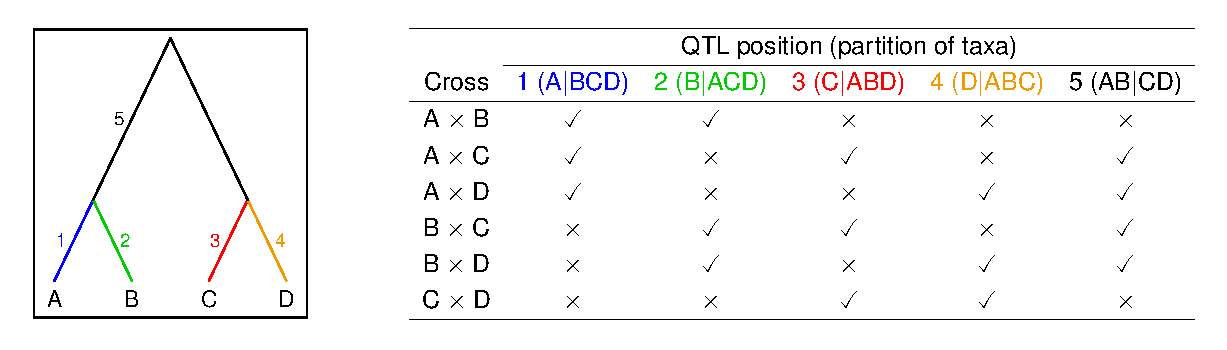
\includegraphics[width=\textwidth]{Figs/fig1.eps}

\vspace{1cm}

\caption{Illustration of the basic concepts behind the mapping of a
  QTL to a phylogenetic tree.  On the left is an example tree
  relating four taxa.  The locations of possible origins of a
  diallelic QTL are indicated by the numbers 1--5.  In the table on
  the right, we indicate the presence or absence of a QTL in each of
  the six possible crosses among pairs of taxa, according to the
  location of the QTL on the tree.  Each possible QTL location on the
  tree corresponds to a partition of the taxa into two
  groups.\label{fig:tree}}
\end{figure}


\newpage
\begin{figure}
\centering
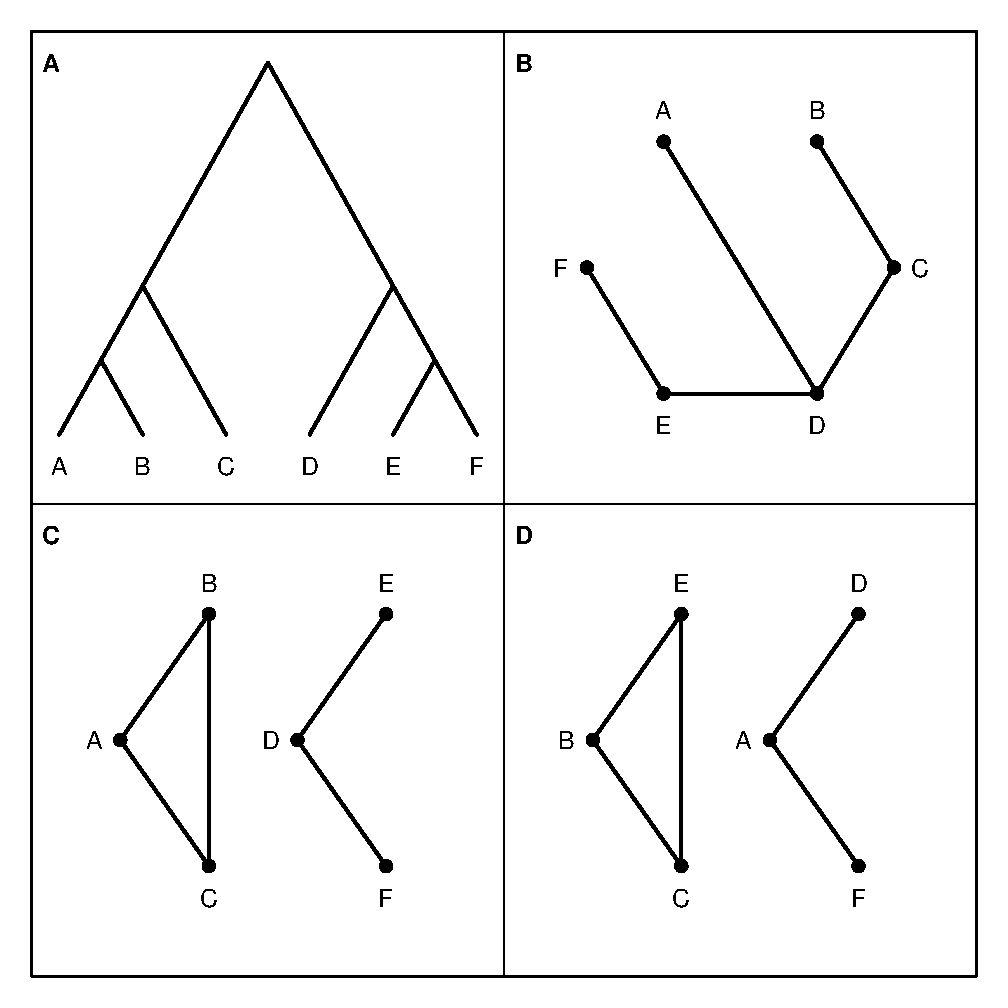
\includegraphics[width=\textwidth]{Figs/fig2.eps}

\vspace{1cm}

\caption{A phylogenetic tree with six taxa (A) and three possible choices of
  five crosses among the six taxa (B--D), with nodes denoting taxa and edges
  denoting crosses.\label{fig:sixtaxa}}
\end{figure}


\newpage
\begin{figure}
\centering
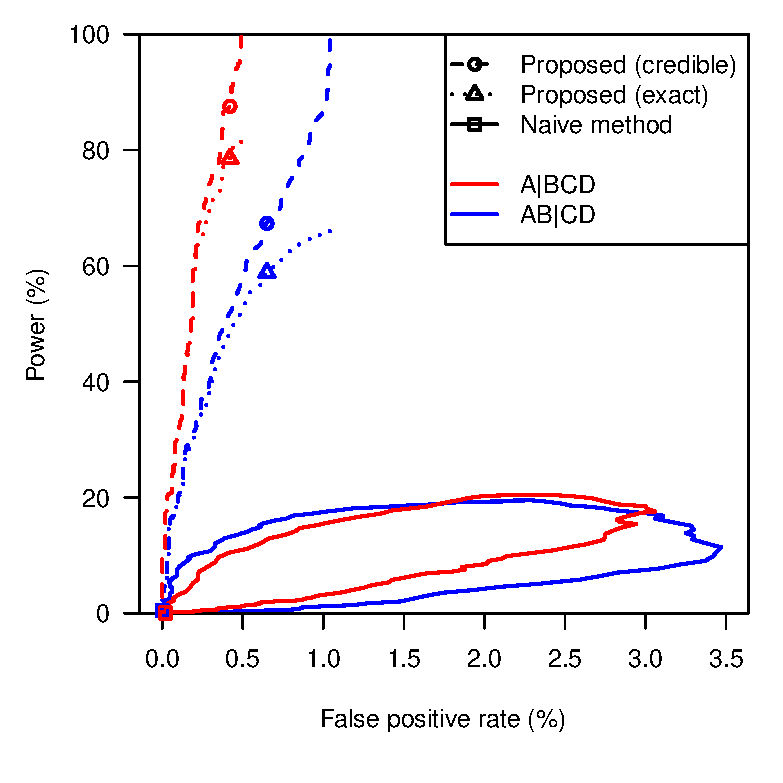
\includegraphics[width=\textwidth]{Figs/fig3.eps}

\vspace{1cm}

\caption{Estimated receiver operating characteristic (ROC) curves for the
  naive method (solid curves), the proposed method, with power
  indicating that true
  partition is contained within 95\% credible
  set (dashed curves), and the proposed method, with power indicating
  that the 95\% credible set contains only the true partition (dotted curves), 
  in the case of four taxa, with each of the six possible intercrosses
  having a sample size of 75, and a QTL responsible for 10\% of the
  phenotypic variance in the crosses in which it is segregating.  The
  red and blue curves correspond to the case that the true partition is
  A$|$BCD and AB$|$CD, respectively.  Dots indicate the power and
  false positive rates for a 5\% significance threshold.  The results are based on
  10,000 simulation replicates.\label{fig:roc}}
\end{figure}


\newpage
\begin{figure}
\centering
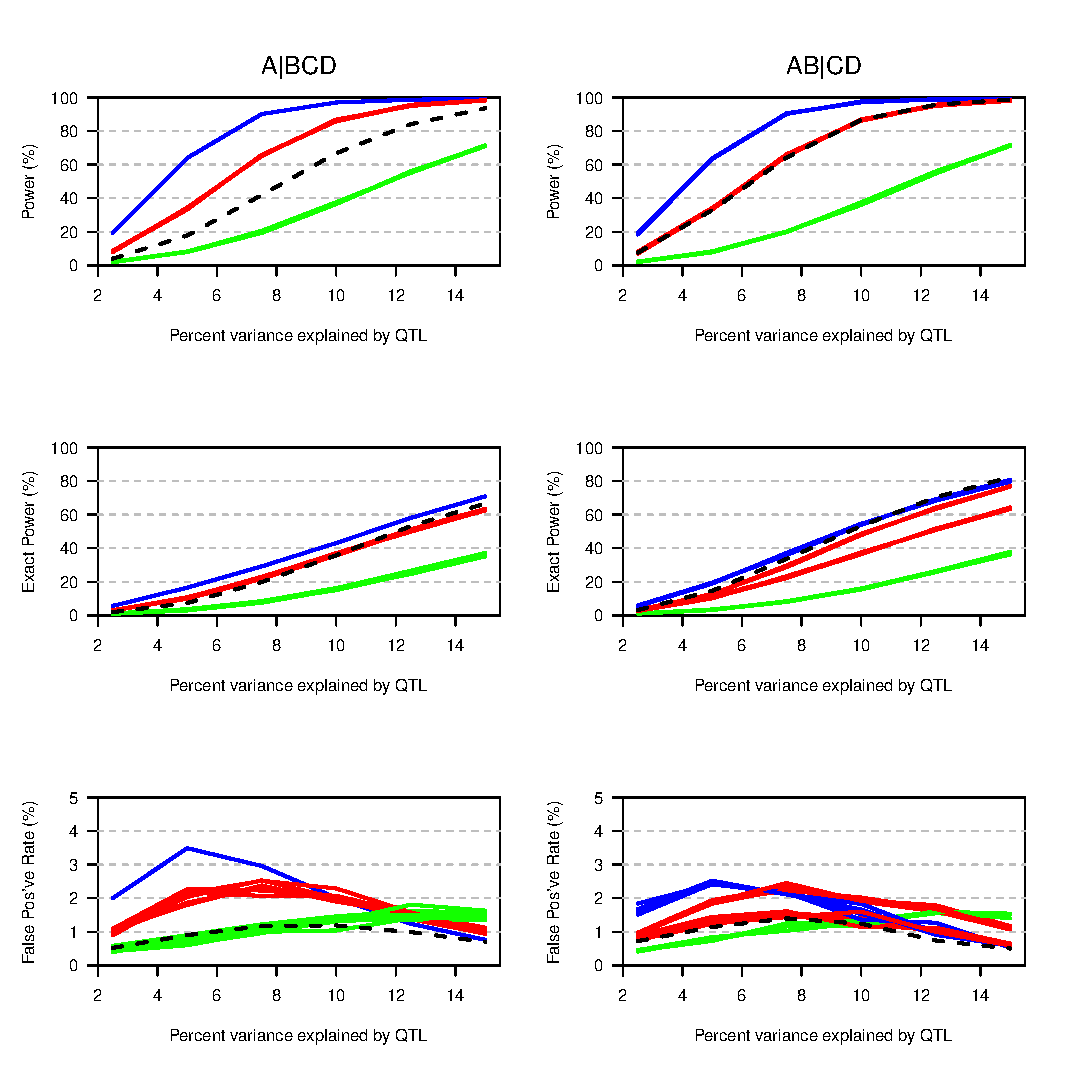
\includegraphics[width=\textwidth]{Figs/fig4.eps}

\vspace{1cm}

\caption{Estimated power (top panels), ``exact'' power (middle panels)
  and false positive rates (bottom panels) in the case of four taxa
  with a total sample size of 450, as a function of the percent
  phenotypic variance explained by the QTL.  The black dashed curves
  correspond to the use of all six possible crosses.  The other curves
  are for the various choices of a minimal set of three crosses, with
  the curves in blue, red and green corresponding to cases in which 3,
  2 and 1 of the crosses are segregating the QTL, respectively.  The
  results are based on 10,000 simulation replicates, with analyses
  considering all possible partitions of the taxa.\label{fig:power}}
\end{figure}


\newpage
\begin{figure}
\centering
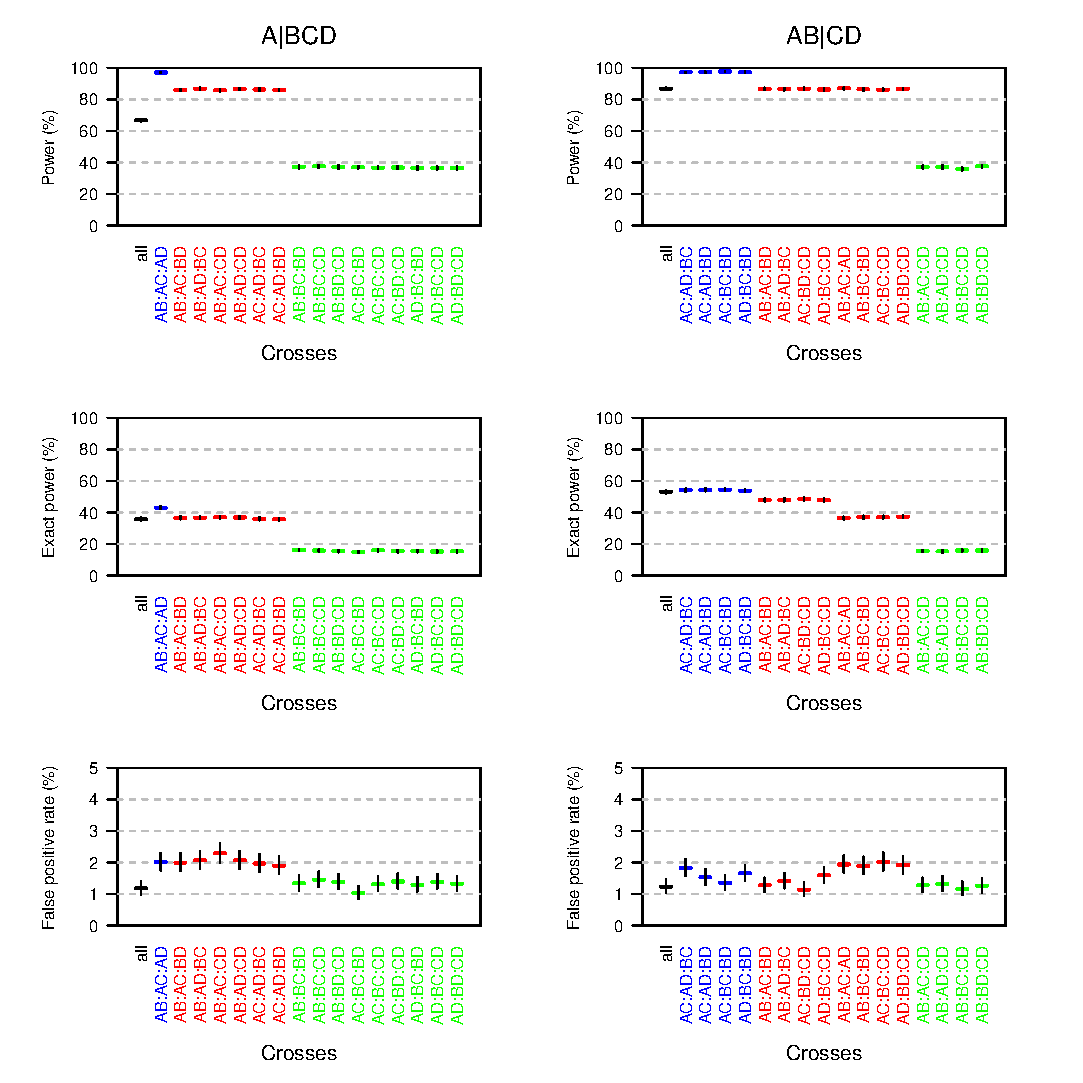
\includegraphics[width=\textwidth]{Figs/fig5.eps}

\vspace{1cm}

\caption{Detailed results on the estimated power (top panels),
  ``exact'' power (middle panels) and false positive rates (bottom
  panels), for individual choices of crosses, in the case of four taxa
  with a total sample size of 450, and with the QTL being responsible
  for 10\% of the phenotypic variance in crosses in which it is
  segregating. Blue, red and green correspond to cases in which 3, 2,
  and 1 of the crosses are segregating the QTL, respectively.  The
  results are based on 10,000 simulation replicates, with analyses
  considering all possible partitions of the taxa.  The black vertical
  line segments indicate 95\% confidence
  intervals.\label{fig:detailedpower}}
\end{figure}


\newpage
\begin{figure}
\centering
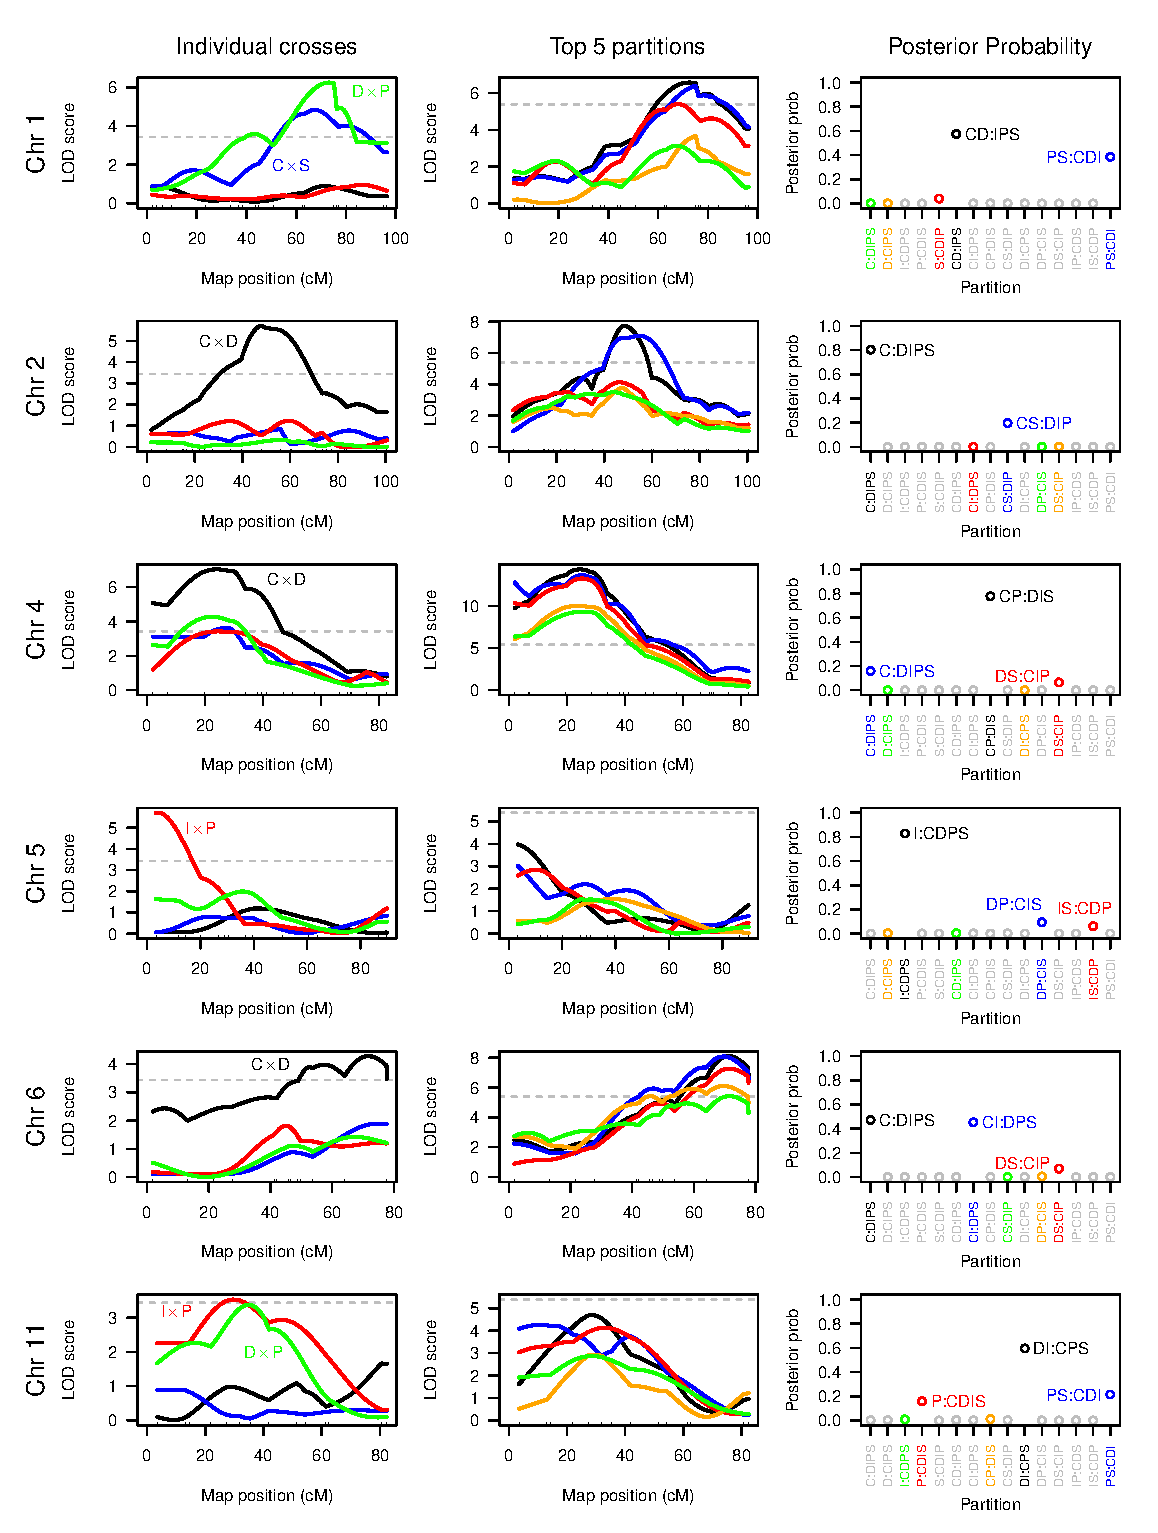
\includegraphics[width=6.2in]{Figs/fig6.eps}

\vspace{5mm}

\caption{Application results (see legend on pg~\pageref{fig6legend}).\label{fig:app}}
\end{figure}


\end{document}
